\documentclass[letterpaper,12pt]{article}
\usepackage[utf8]{inputenc}
\usepackage{geometry}
\usepackage{amsmath}
\usepackage{float}
\usepackage{graphicx}
\usepackage{subcaption}
\usepackage{amssymb}
\usepackage{adjustbox}
\usepackage{wrapfig} %%imagen envuelta por un texto
\usepackage{xcolor}
\usepackage{fancyhdr}

\title {\textbf{"Geometría Analítica"}}
\author{Deniso Xocuis}
\date{26 de marzo de 2023}
\geometry{top=2cm, bottom=2cm, left=2cm, right= 2cm} %%margen
\graphicspath{{images/}}
\parindent=0pt

\begin{document}
\maketitle
\thispagestyle{empty}
\newpage
\setcounter{page}{1}
\pagestyle{headings}

%%%%%%%%%%%%%%%%%%%%%%%%%%%%%%%%%VECTORES EN 2D%%%%%%%%%%%%%%%%%%%%%%%%%%%%%%%%
\begin{sloppypar} %%%%para que esté todo justificado 
\section{Operaciones con vectores}
\subsection{Vectores en 2D}
\noindent Los \emph{vectores} se pueden multiplicar, sumar o restar, pueden crearse nuevos vectores dependiendo la operación necesaria. En muchas aplicaciones de los vectores es útil \emph{encontrar un vector que tenga la misma dirección que un vector dado.} Los \textbf{vectores unitarios} tienen longitud 1 y la misma dirección que $\vec{v}$, ayudan a darle \textbf{dirección} ($\theta$) a un punto. El proceso de multiplicar $\vec{v}$ por 1/$\| \vec{v} \|$ para obtener un vector unitario se llama \textbf{normalización de $\vec{v}$}

\begin{center}
    
    $\displaystyle \vec{u} = \frac{\vec{v}}{\| \vec{v} \|}$, \textcolor[rgb]{1,0,0}{(\textbf{\textit{vector unitario en la dirección de v}})}
\end{center}
\noindent Fórmulas generales para vectores:
\begin{center}
    
    $\theta$ = $\displaystyle \cos^{-1}$ ($\displaystyle \frac{V_n}{\| \vec{V} \Vert }$)
    
    \textcolor[rgb]{1,0,0} {(\textbf{\textit{cálculo del ángulo}})}
   \vspace{0.3cm}\\
    $V_x$ =  $\| {V} \Vert  \cos \theta$; $V_y = \|{V}\vert \sin \theta$  
    
    \textcolor[rgb]{1,0,0}{(\textbf{\textit{descomposición o combinación lineal de un vector en componentes unitarios}})}

\end{center}

%%%%%%%%%%%%%%%%%%%%%%%%%%%%%%%%%%%%%vectores unitarios%%%%%%%%%%%%%%%%%%%%%%%%
\subsection{Vectores unitarios canónicos o estándar}
\noindent A los vectores unitarios $<1,0>$ y $<0,1>$ se les llama vectores unitarios canónicos o estándar en el plano y se denotan por: $\hat{i} = <1,0 >$ y $\hat{j} = <0,1>$.

\begin{center}
    $u = \cos \theta \hat{i} + \sin \theta \hat{j}$   \textcolor[rgb]{1,0,0}{(\textbf{\textit{vector unitario}})}
\end{center}

\noindent Al vector $\vec{v} = v_1\hat{i} + v_2\hat{j}$ se le llama \textbf{combinación lineal} de $\hat{i}$ y $\hat{j}$. A los escalares $v_1$ y $v_2$ se les llama \textbf{componentes horizontal y vertical} de v. \textbf{La magnitud debe ser igual a 1.}



\begin{center}
    v = $\| v \| \mu $
    
    \textcolor[rgb]{1,0,0}{(\textbf{\textit{descomposición de un vector por vector unitario}})}
\end{center}


%%%%%%%%%%%%%%%%%%%%%%%%%%%%%%%%%%%%%%VECTORES EN 3D%%%%%%%%%%%%%%%%%%%%%%%%%%%
\subsection{Vectores en 3D}
\noindent En el espacio los vectores se denotan mediante ternas ordenadas $\vec{v}$ = <$v_1,v_2,v_3$>. Usando los vectores unitarios $\hat{i}= \langle1,0,0\rangle, \hat{j}=\langle 0,1,0\rangle$  y  $\hat{k}=\langle 0,0,1\rangle$, la notación empleando los vectores unitarios canónicos o estándar para $\vec{v}$ es muy similar a la notación en el plano.
\begin{center}
    
    $\vec{v} = v_1\hat{i} + v_2\hat{j}+v_3\hat{k}$
    
\end{center}

\noindent Los \textcolor[rgb]{1,0,0}{\textbf{\textit{cosenos directores}}} se obtienen mediante el uso de funciones trigonométricas.
\begin{center}
    $\displaystyle \alpha = \cos^{-1} \frac{x_2-x_1}{\| \vec{v} \| }$ = $\displaystyle \cos^{-1} \frac{v_x}{\| \vec{v} \| }$
    
    $\displaystyle \beta = \cos^{-1} \frac{y_2-y_1}{\| \vec{v} \| }$ = $\displaystyle \cos^{-1} \frac{v_y}{\| \vec{v} \| }$
    
    $\displaystyle \gamma = \cos^{-1} \frac{z_2-z_1}{\| \vec{v} \| }$ = $\displaystyle \cos^{-1} \frac{v_z}{\| \vec{v} \| }$
    \vspace{0.3cm}\\
    \noindent Estos ángulos directores poseen las siguiente propiedad:
    \vspace{0.3cm}\\
    $\cos ^{2} \alpha + \cos ^{2} \beta + \cos ^{2} \gamma$ = 1
\end{center}

%%%%%%%%%%%%%%%%%%%%%%%%%%%%%%%%%%%FUERZAS%%%%%%%%%%%%%%%%%%%%%%%%%%%%%%%%%%%%
\section{Fuerzas}
\subsection{Fuerzas en 3D}
\begin{center}
    $\vec{F} = \|F\| \mu$  \textcolor[rgb]{1,0,0}{(\textbf{\textit{descomposición de una fuerza}})} 
    \vspace{0.3cm}\\
    $\displaystyle \mu_{MN} = \frac{MN}{\|MN\|}$
    \vspace{0.3cm}\\
    $\displaystyle \cos \alpha = \frac{T_{MNx}}{\|T_{MN}\|}$ ; $\displaystyle \cos \beta = \frac{T_{MNy}}{\|T_{MN}\|}$ ; $\displaystyle \cos \gamma = \frac{T_{MNz}}{\|T_{MN}\|}$
    \vspace{0.3cm}\\
    Para \textbf{tensiones}, las fórmulas son las mismas ya que estamos hablando de fuerzas.
\end{center}
\noindent \textbf{EJEMPLO 1}: Determine la representación vectorial de la fuerza de 240 N en compontentes rectangulares.
\begin{figure}[H]
    \centering
     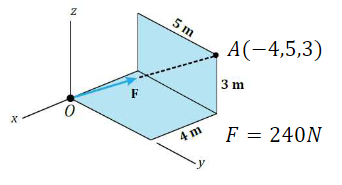
\includegraphics[width=0.4\textwidth]{images/vector.PNG}
\end{figure}
\noindent La representación vectorial de una fuerza significa representarla por ordenadas usando los vectores unitarios teniendo en cuenta su dirección, para eso lo que hacemos es multiplicar la magnitud por el vector unitario.

\begin{center}
    $\|A\| = 5\sqrt{2}$ $\therefore$ $\displaystyle \mu$ = $\displaystyle \frac{-4\hat{i}+5\hat{j}+ 3\hat{k}}{5\sqrt{2}}$
    \vspace{0.3cm}\\
    $\vec{F}$ = 240$\displaystyle (\frac{-4\hat{i}+5\hat{j}+ 3\hat{k}}{5\sqrt{2}})$
    \vspace{0.3cm}\\
    $\therefore$ la representación vectorial es: $\vec{F}$ = $(135.8\hat{i}+169.7\hat{j}+101.82\hat{k})N$
\end{center}

%%%%%%%%%%%%%%%%%%%%%%%%%%%%%%%%%%VECTORES PARALELOS%%%%%%%%%%
\section{Vectores paralelos}
\noindent Los múltiplos escalares positivos de un vector $\vec{v}$ tienen la misma dirección que $\vec{v}$, los múltiplos negativos tienen la dirección opuesta. 

\noindent Dos vectores son \textbf{paralelos} si existe algún escalar \textit{c} tal que $\vec{u}$= c$\vec{v}$, simbólicamente se representa como $\vec{u} \| \vec{v} $.

\noindent Los vectores \textbf{paralelos} forman un ángulo de 0°. Los vectores \textbf{antiparalelos} forman un ángulo de 180°.

\begin{figure}[H]
    \centering
    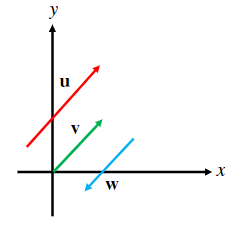
\includegraphics[width=0.4\textwidth]{images/vecpar.PNG}
\end{figure}
\noindent De acuerdo a la figura, se concluye lo siguiente:
\begin{itemize}
    \item Los vectores $\vec{u}$ y $\vec{v}$ son \textbf{paralelos entre sí}, si $\vec{u} \| \vec{v}$ (ángulo de 0°)
    \item Los vectores $\vec{v}$ y $\vec{w}$ son \textbf{antiparalelos entre sí}, si $\vec{u} \uparrow \downarrow  \vec{v}$ (ángulo de 180°), pasa lo mismo con $\vec{u}$ y $\vec{w}$
\end{itemize}


\textbf{EJEMPLO:}

\noindent El vector $\vec{w}$ tiene punto inicial (2,-1,3) y punto final (-4,7,5). ¿Cuál de los vectores siguientes es paralelo a $\vec{w}$?

\noindent Iniciamos sacando la distancia total del vector $\vec{w}$, es decir, la distancia del punto A y el punto B.

\begin{center}
    $\vec{AB}$ = $<(-4-2),(7+1),(5-3)>$ = $-6,8,2$
\end{center}

\begin{center}
    ¿$\vec{u} = <3,-4,-1>$ es $\|$ a $\vec{w}$?
    \vspace{0.3cm}\\
    $\displaystyle \frac{-6}{3}$ = $\displaystyle \frac{8}{-4}$ = $\displaystyle \frac{2}{-1}$
    \vspace{0.3cm}\\
    $\therefore$ -2 = -2 = -2, la constante es "-2", eso quiere decir que son \textbf{antiparalelos}
\end{center}

%%%%%%%%%%%%%%%%%%%%%%%%%%PRODUCTO PUNTOO%%%%%%%%%%%%%%%%%%%%%%%%%%%%%%%%%%%

\section{Producto punto o escalar}
\noindent Combinación de dos vectores, la expresión es un escalar, también es llamado producto interno.

\noindent Ejemplo:

\noindent dados $\vec{\mu} = <2,-2>$, $\vec{v} = <5,8>$, encontrar su producto punto.

= (2)(5) + (-2)(8) = 10-16=-6

\noindent Gracias a esto se puede saber si \textbf{dos vectores son ortogonales(perpendiculares) si su producto punto es igual a cero.}

\subsection{Forma alternativa}
\noindent También se puede sacar el producto escalar de dos vectores de la siguiente manera:

\begin{center}
    u$\cdot$v = $\|u\| \|v\| \cos\theta $
\end{center}
\section{Ángulo entre dos vectores}
\noindent La fórmula es la siguiente:

\begin{center}
    $\displaystyle \cos \theta = \frac{\vec{\mu}\cdot\vec{v}}{\|\vec{\mu}\| \|\vec{v}\|}$
\end{center}

%%%%%%%%%%%%%%%%%%%%%%%TRABAJO%%%%%%%%%%%%%%%%%%%%%%%%%%%%%%%%%%%%%%

\section{Trabajo: Aplicaciones del producto punto}
\noindent El producto escalar del vector fuerza por el vector desplazamiento. 

\begin{center}
    $W = \|proy_{\vec{PQ}}\textbf{F}\| \|\vec{PQ}\|$ \textcolor[rgb]{1,0,0}{(\textbf{\textit{en forma de proyección}})}
    \vspace{0.3cm}\\
    $W = \textbf{F} \cdot \vec{PQ}$ \textcolor[rgb]{1,0,0}{(\textbf{\textit{en forma de producto escalar}})} 
\end{center}
\subsection{Ejemplo 1}
\noindent Una fuerza $\vec{F}$= (6$\hat{i}$ - 2$\hat{j}$)N actúa sobre una partícula que experimenta un desplazamiento $\Delta \vec{r}$ = (3$\hat{i}$ + $\hat{j}$) m. Encuentre el trabajo realizado por la fuerza sobre la partícula y el ángulo entre la fuerza y el incremento del desplazamiento.
\vspace{0.3cm}\\
$\vec{F}$= (6$\hat{i}$ - 2$\hat{j}$)N   ;   $\|\vec{F} \|$ = $\sqrt{40}$
\vspace{0.3cm}\\
$\vec{r}$ = (3$\hat{i}$ + $\hat{j}$) m  ;   $\|\Delta\vec{r}\| = \sqrt{10}$
\vspace{0.3cm}\\
$\therefore W= \vec{F} \cdot \vec{r}$ = 16 J
\subsection{Ejemplo 2}
\noindent La fuerza tiene una magnitud de $\vec{F_{p}}$=100 N y forma un ángulo de 37° con el suelo. Calcule el trabajo realizado por esta fuerza cuando el cajón se jala 40m a lo largo del suelo.
\vspace{0.3cm}\\
$\|\vec{F_{p}}\|$=100 N 
\vspace{0.3cm}\\
$\vec{F_{p}} = (100 \cos 37$° + $100 \sin 37$°) N
\vspace{0.3cm}\\
$\vec{F_{p}} = (79.86 \hat{i} + 60.18 \hat{j}) N$
\vspace{0.3cm}\\
W= 3.194kJ
\newpage
%%%%%%%%%%%%%%%%%%%%%%%%%%%%PROYECCIÓN DE VECTORES%%%%%%%%%%%%%%

\section{Proyección de vectores}
\noindent Sean $\vec{u}$ y $\vec{v}$ vectores distintos de cero. Sea $\vec{u} = w_1 + w_2$ \textbf{donde $w_1$ es paralelo a $\vec{v}$ y $w_2$ es ortogonal a $\vec{v}$.}
\begin{enumerate}
    \item A $w_1$ se le llama la \textbf{\textit{proyección de $\vec{u}$ en $\vec{v}$}} o la componente vectorial de $\vec{u}$ a lo largo de $\vec{v}$ y se denota por $w_1 = proy_{\vec{v}}\vec{u}$
    \item A $w_2$ = $\vec{u} - \vec{w_1}$, se le llama la \textbf{\textit{componente vectorial de $\vec{u}$ ortogonal a $\vec{v}$}}
\end{enumerate}

\begin{figure}[H]
    \centering
    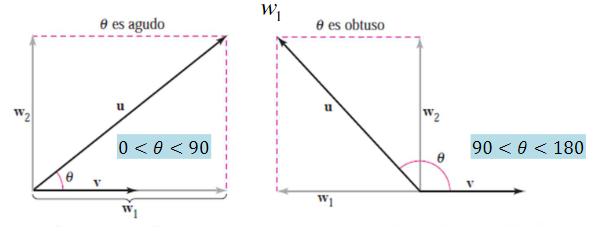
\includegraphics{images/proyc.PNG}
\end{figure}
\noindent \textbf{Proyección de $\vec{u}$ sobre $\vec{v}$:}

$Proy_v\vec{u}$

\noindent Se puede entender como la sombra que proyecta el vector $\vec{u}$ sobre el vector $\vec{v}$

\begin{center}
    $\displaystyle proy_{v}\vec{u} = \frac{u\cdot v}{\|v \|^2} v$
    \vspace{0.3cm}\\
    $\displaystyle proy_{u}\vec{v} = \frac{u\cdot v}{\|u \|^2} u$
\end{center}

%%%%%%%%%%%%%%%%%%PRODUCTO VECTORIAL DE VECTORES EN EL ESPACIO
\section{Producto vectorial de vectores en el espacio}
\noindent Es necesario encontrar un vector en el espacio \textbf{ortogonal (perpendicular)} a dos vectores dados que forman un plano. 

\noindent El producto vectorial de dos vectores en el espacio se define y calcula utilizando los vectores unitarios canóninos por medio de PRODUCTO CRUZ. La manera de calcular u x v es con la \textbf{\textit{Regla de Laplace}}

\subsection{Aplicación: Cálculo del área}
Es necesario conocer dos longitudes de un paralelogramo para calcular su área

\subsection{Aplicación: Física/Estática}
El producto vectorial puede utilizarse para medir el \textbf{momento(torque) M de una Fuerza F respecto a un punto P}. Si el punto de aplicación de la fuerza es Q, el momento de \textbf{F} respecto a P está dado por:

\begin{center}
    \textbf{M = PQ x F} (momento de F respecto a P)
\end{center}
\section{Triple producto escalar (o producto mixto)}
\noindent La fórmula es:

\begin{center}
    $u \cdot (v \times  w) = \begin{pmatrix}
        u_1 & u_2 & u_3\\ 
        v_1 & v_2 & v_3\\ 
        w_1 & w_2 & w_3
    \end{pmatrix}$
\end{center}
\noindent El triple producto escalar puede usarse para determinar el volumen del paralelepípedo con u,v y w como aristas. 
\section{Coordenadas cilíndricas}
Para ver primero lo que son coordenadas cilíndricas hay que primero ver que son las coordenadas polares.
\subsection{Coordenadas polares}
Acá ya no tenemos proyecciones en el eje x o en el eje y, tenemos lo que se llama un polo de origen y un eje llamado "eje polar", llamado como:
\begin{center}
    \textbf{$(r, \theta)$} donde:
    r = distancia dirigida de O a p
    $\theta$ = ángulo dirigido desde el eje polar hasta el segmento OP

\end{center}






%%%%%%%%%%%%%%%%%%%%%%%%%%%%%%%%%%%MAPLEEE%%%%%%%%%%%%%%%%%%%%%%%%%%%%%%%%%%%
\section{Maple}
\begin{center}
    Siempre se debe comenzar de la siguiente forma:
\end{center}
\noindent $>$ \textcolor[rgb]{1,0,0}{restart;} \textit{(nota: siempre se termina con un punto y coma)}

\noindent $>$ \textcolor[rgb]{1,0,0}{with(linalg);} \textit{(esto sirve para las librerías)}
\begin{center}
    Para definir un vector usamos los intervalos, sirve para 2D y 3D, ejemplo:
\end{center}
\noindent $>$ \textcolor[rgb]{1,0,0}{u:=vector([1,2,3]);} 

\begin{center}
    \textcolor{blue}{u:=([1,2,3])}
\end{center}

%%%%%%%%%%%%%%%%%%%%%%%%%%%%FORMULARIO%%%%%%%%%%%%%%%%%%%%%
\newpage
\centering
\section*{\textbf{FORMULARIO}}
\subsection*{\textbf{Vectores en 2D}}
$\displaystyle \vec{\mu} = \frac{\vec{v}}{\| \vec{v} \|}$, \textcolor[rgb]{0.2,0.5,0.7}{\textbf{\textit{(vector unitario en la dirección de v)}}}
\vspace{0.3cm}\\
$\vec{\mu} = <\cos \theta, \sin \theta>$ = $\cos \theta\hat{i}, \sin \theta\hat{j}$ \textcolor[rgb]{0.2,0.5,0.7}{\textbf{\textit{(vector unitario)}}}
\vspace{0.3cm}\\
$\vec{v} = \|v\|\cos \theta\hat{i} + \|v\|\sin \theta\hat{j}$ \textcolor[rgb]{0.2,0.5,0.7}{\textbf{\textit{(descomponer un vector)}}}
\vspace{0.3cm}\\
Es lo mismo que decir:

$v_x = \|v\| \cos\theta$ \hspace{0.4cm} $v_y = \|v\| \cos\theta$

\subsection*{\textbf{Vectores en 3D}}
\textcolor[rgb]{0.2,0.5,0.7}{\textbf{\textit{cosenos directores:}}}

$\displaystyle \alpha = \cos^{-1} \frac{x_2-x_1}{\| \vec{v} \| }$ = $\displaystyle \cos^{-1} \frac{v_x}{\| \vec{v} \| }$
    
$\displaystyle \beta = \cos^{-1} \frac{y_2-y_1}{\| \vec{v} \| }$ = $\displaystyle \cos^{-1} \frac{v_y}{\| \vec{v} \| }$
    
$\displaystyle \gamma = \cos^{-1} \frac{z_2-z_1}{\| \vec{v} \| }$ = $\displaystyle \cos^{-1} \frac{v_z}{\| \vec{v} \| }$
\vspace{0.3cm}\\  
$\cos ^{2} \alpha + \cos ^{2} \beta + \cos ^{2} \gamma$ = 1 \textcolor[rgb]{0.2,0.5,0.7}{\textbf{\textit{(propiedad)}}}

$\vec{v} = \|v\|\mu$ \textcolor[rgb]{0.2,0.5,0.7}{\textbf{\textit{(descomponer un vector 3D)}}}

\subsection*{\textbf{Fuerza resultante en 2D}}
$F_n = \|F\|<\cos \theta,\sin \theta>$ \textcolor[rgb]{0.2,0.5,0.7}{\textbf{\textit{(descomponer una fuerza en 2D)}}}
\vspace{0.3cm}\\
$F_R = F_1 + F_2$ \textcolor[rgb]{0.2,0.5,0.7}{\textbf{\textit{(fuerza resultante)}}}

\subsection*{\textbf{Fuerza resultante en 3D}}
\textit{nota: la fuerza también es llamada "tensión", el peso es independiente}
\vspace{0.3cm}\\
$F = \|F\|\mu$ \textcolor[rgb]{0.2,0.5,0.7}{\textbf{\textit{(descomponer una fuerza en 3D)}}}
\vspace{0.3cm}\\
$\vec{T_{AB}} = \| \vec{T_{AB}}\| \mu_{AB}$ \textcolor[rgb]{0.2,0.5,0.7}{\textbf{\textit{(descomponer la tensión)}}}

\subsection*{\textbf{Producto punto : forma alternativa}} 
$u \cdot v = \|u\| \|v\| \cos \theta$ 

\subsection*{\textbf{Ángulo entre vectores}}
$\displaystyle \cos \theta = \frac{u \cdot v}{\|u\| \|v\|}$

\subsection*{\textbf{Trabajo}}
$W = \|proy_{PQ}\textbf{F} \|\vec{PQ}\|$ 
\vspace{0.3cm}\\
$W = \textbf{F} \cdot \vec{PQ}$

\subsection*{\textbf{Proyección de vectores}}
$\vec{u} = w_1+w_2$
\vspace{0.3cm}\\ 
$w_1 = proy_{v}\vec{u}$
\vspace{0.3cm}\\ 
$w_2 = \vec{u} - w_1$
\vspace{0.3cm}\\ 
$\displaystyle proy_{v}\vec{u} = \frac{u \cdot v}{\|v\|^2} v$ 

\subsection*{\textbf{Momento(torque)}}
$M_o = \vec{r} \times F$ o $M_o = \vec{PQ} \times F$


%%%%%%%%%%%%%PASOS DESCRIPTIVOS
\newpage
\section*{Reglas generales de los sistemas}
\textit{sin mecanizar los pasos}
\subsection*{Encontrar un vector con magnitud y dirección dada en 3D}
\begin{enumerate}
    \item Sacar vector unitario a el vector de dirección 
    \item Multiplicar la magnitud por esa dirección siguiendo las fórmulas de descomposición de vectores
\end{enumerate}
\subsection*{Encontrar los componentes de un vector con magnitud y ángulo en 3D}
\begin{enumerate}
    \item Descomponer el ángulo por coseno y seno
    \item Multiplicar la magnitud por las direcciones siguiendo las fórmulas de descomposición de vectores 
\end{enumerate}
\subsection*{Hallar las componentes de un vector unitario por magnitud dada}
\begin{enumerate}
    \item Sacar las componentes del vector de dirección
    \item Seguir los pasos de "encontrar un vector con magnitud y dirección dada en 3D"
\end{enumerate}
\subsection*{Fuerzas/tensiones en 3D}
\begin{enumerate}
    \item Ubicar las componentes de cada punto
    \item Sacar distancias de cada punto correspondiente que nos pidan 
    \item Sacar el vector unitario de la longitud de el punto de tensión que nos pidan 
    \item Multiplicar la magnitud de la fuerza de tensión por el vector unitario 
\end{enumerate}
\textit{En caso de que nos den el peso y no la fuerza de tensión, para encontrar las tensiones es lo siguiente:}
\begin{enumerate}
    \item Multiplicar cada tensión por el vector unitario dado 
    \item Realizar un sistema de ecuaciones
    \item Resolver por "sustitución"
\end{enumerate}
\section*{Momento}
\begin{enumerate}
    \item Ubicar las componentes de la fuerza, si la fuerza es al rededor de una distancia, es necesario descomponer esa fuerza.
    \item Sacar la distancia del vector $\vec{PQ}$ con las fórmulas de descomposición de vectores, si nos piden determinar el momento de fuerza al rededor de x ejercida desde el punto y, será un vector $\vec{xy}$ 
    \item Realizar producto vectorial
\end{enumerate}












\end{sloppypar}
\end{document}